\section{ComponentManager Klassenreferenz}
\label{classComponentManager}\index{ComponentManager@{ComponentManager}}
Klassendiagramm für ComponentManager::\begin{figure}[H]
\begin{center}
\leavevmode
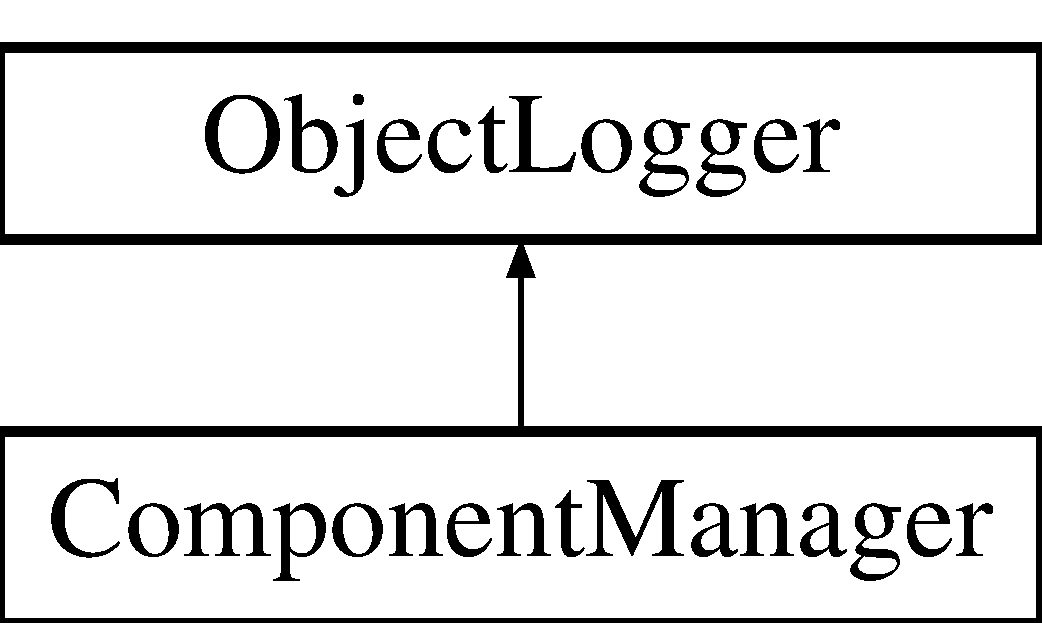
\includegraphics[height=2cm]{classComponentManager}
\end{center}
\end{figure}
\subsection*{Öffentliche Methoden}
\begin{CompactItemize}
\item 
{\bf ComponentManager} ()
\item 
{\bf getComponent} (\$className, \$instanceName, \&\$smartyObj)
\item 
{\bf loadComponents} ()
\item 
{\bf \_\-getUID} (\$length)
\item 
{\bf \_\-assign\_\-rand\_\-value} (\$num)
\end{CompactItemize}
\subsection*{Öffentliche Attribute}
\begin{CompactItemize}
\item 
{\bf \$\_\-instancesArr}
\item 
{\bf \$\_\-instancesKeysArr}
\item 
{\bf \$\_\-idLenght} = 4
\end{CompactItemize}


\subsection{Ausführliche Beschreibung}


Definiert in Zeile 9 der Datei class.ComponentManager.php.

\subsection{Dokumentation der Elementfunktionen}
\index{ComponentManager@{ComponentManager}!ComponentManager@{ComponentManager}}
\index{ComponentManager@{ComponentManager}!ComponentManager@{ComponentManager}}
\subsubsection{\setlength{\rightskip}{0pt plus 5cm}ComponentManager.ComponentManager ()}\label{classComponentManager_03aadeb58f4514bf579786ed60f36c0e}




Definiert in Zeile 16 der Datei class.ComponentManager.php.\index{ComponentManager@{ComponentManager}!getComponent@{getComponent}}
\index{getComponent@{getComponent}!ComponentManager@{ComponentManager}}
\subsubsection{\setlength{\rightskip}{0pt plus 5cm}ComponentManager.getComponent (\$ {\em className}, \$ {\em instanceName}, \&\$ {\em smartyObj})}\label{classComponentManager_ad16dcb2419e0e7c3004693064aaf62f}


Get instance of component

\begin{Desc}
\item[Parameter:]
\begin{description}
\item[{\em string}]\$className \end{description}
\end{Desc}


Definiert in Zeile 30 der Datei class.ComponentManager.php.

Benutzt \_\-getUID().\index{ComponentManager@{ComponentManager}!loadComponents@{loadComponents}}
\index{loadComponents@{loadComponents}!ComponentManager@{ComponentManager}}
\subsubsection{\setlength{\rightskip}{0pt plus 5cm}ComponentManager.loadComponents ()}\label{classComponentManager_7b007b47d8301ba0df504d5cd4589544}


Load required components

\begin{Desc}
\item[Rückgabe:]bool \end{Desc}


Definiert in Zeile 64 der Datei class.ComponentManager.php.

Benutzt ObjectLogger.\_\-addError() und ObjectLogger.\_\-resetErrors().\index{ComponentManager@{ComponentManager}!\_\-getUID@{\_\-getUID}}
\index{\_\-getUID@{\_\-getUID}!ComponentManager@{ComponentManager}}
\subsubsection{\setlength{\rightskip}{0pt plus 5cm}ComponentManager.\_\-getUID (\$ {\em length})}\label{classComponentManager_74032b7e41d550f35833ff1ca1d25e77}


Get unic UID with length \$length  private \begin{Desc}
\item[Parameter:]
\begin{description}
\item[{\em long}]\$length \end{description}
\end{Desc}
\begin{Desc}
\item[Rückgabe:]string \end{Desc}


Definiert in Zeile 100 der Datei class.ComponentManager.php.

Benutzt \_\-assign\_\-rand\_\-value().

Wird benutzt von getComponent().\index{ComponentManager@{ComponentManager}!\_\-assign\_\-rand\_\-value@{\_\-assign\_\-rand\_\-value}}
\index{\_\-assign\_\-rand\_\-value@{\_\-assign\_\-rand\_\-value}!ComponentManager@{ComponentManager}}
\subsubsection{\setlength{\rightskip}{0pt plus 5cm}ComponentManager.\_\-assign\_\-rand\_\-value (\$ {\em num})}\label{classComponentManager_d89866f2f3e17789cb467aeb08d2f0d7}


get char by bumber

\begin{Desc}
\item[Parameter:]
\begin{description}
\item[{\em long}]\$num \end{description}
\end{Desc}
\begin{Desc}
\item[Rückgabe:]string \end{Desc}


Definiert in Zeile 118 der Datei class.ComponentManager.php.

Wird benutzt von \_\-getUID().

\subsection{Dokumentation der Datenelemente}
\index{ComponentManager@{ComponentManager}!\$\_\-instancesArr@{\$\_\-instancesArr}}
\index{\$\_\-instancesArr@{\$\_\-instancesArr}!ComponentManager@{ComponentManager}}
\subsubsection{\setlength{\rightskip}{0pt plus 5cm}ComponentManager.\$\_\-instancesArr}\label{classComponentManager_71afde970cdafbfec9dd9026b4b8921c}




Definiert in Zeile 12 der Datei class.ComponentManager.php.\index{ComponentManager@{ComponentManager}!\$\_\-instancesKeysArr@{\$\_\-instancesKeysArr}}
\index{\$\_\-instancesKeysArr@{\$\_\-instancesKeysArr}!ComponentManager@{ComponentManager}}
\subsubsection{\setlength{\rightskip}{0pt plus 5cm}ComponentManager.\$\_\-instancesKeysArr}\label{classComponentManager_ed6a108e9f463cac5f6b3742c882f5c5}




Definiert in Zeile 13 der Datei class.ComponentManager.php.\index{ComponentManager@{ComponentManager}!\$\_\-idLenght@{\$\_\-idLenght}}
\index{\$\_\-idLenght@{\$\_\-idLenght}!ComponentManager@{ComponentManager}}
\subsubsection{\setlength{\rightskip}{0pt plus 5cm}ComponentManager.\$\_\-idLenght = 4}\label{classComponentManager_da83ecf4d685dcd0f24910766d1ee7e8}




Definiert in Zeile 14 der Datei class.ComponentManager.php.

Die Dokumentation für diese Klasse wurde erzeugt aufgrund der Datei:\begin{CompactItemize}
\item 
{\bf class.ComponentManager.php}\end{CompactItemize}
